\begin{figure}
\centering
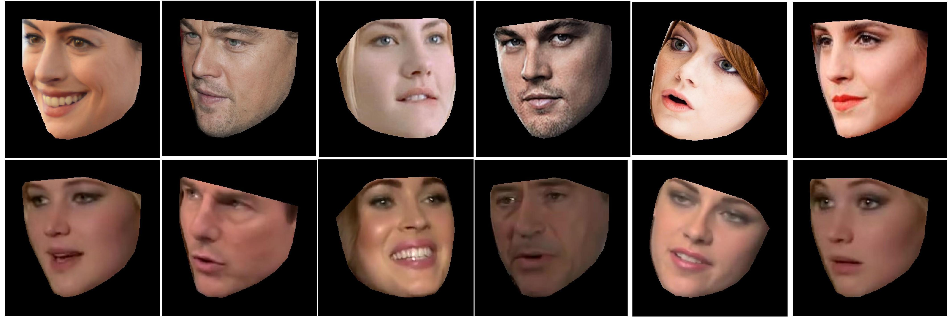
\includegraphics[width =12cm,height=4.2cm]{front/figures/test_exemplar_map.png}
\caption{First row of images are the input profile images. Second row shows the retrieved faces from database.}
\label{fig:test_exemplar_map}
\end{figure}

To retrieve the closest exemplar to the input face, we first need to define a similarity measure between
faces. Let $P^m$ and $P^n$ represent landmarks of two faces. The similarity score between poses of
two faces can then be defined as the Euclidean distance between $P^m$ and $P^n$.
\begin{equation}
    ds^{mn} = \sqrt[2]{\sum_{i=1}^{68}((x_i^m - x_i^n)^2+(y_i^m - y_i^n)^2)} \label{eq:dissimilarity_score}
\end{equation}
However $P^m$ and $P^n$ are defined in different coordinate systems, separated by translation,
rotation and scaling. We need to nullify the effect
of translation and scaling and bring both sets of landmark positions to one coordinate system. 
Note that rotation is not considered as it is one of the parameters of pose and our exemplar database is
exhaustive enough to take care of rotation variations in the input face.
To remove the translational effect, we subtract the mean of $X$ and $Y$ coordinates from both the landmark vectors,
  $X = (X - \mu_X), Y = (Y - \mu_Y)$.
To remove the scaling effect, we multiply $P_m$ by a factor of $s$, given by
\begin{equation}
  s = \frac{\sum_{i=1}^{68}((x_{i}^{m} \times x_{i}^{n})+(y_{i}^{m} \times y_{i}^{n})) }{\sum_{i=1}^{68}((x_{i}^m)^2 + (y_{i}^{m})^2)}  \label{eq:scaling_effect}
\end{equation}
which follows from a straightforward optimization procedure that minimizes \emph{root mean squared
error} (rmse) error between corresponding landmark positions. The derivation is omitted for brevity.

Pose is accurately defined by the position of landmarks on the face. We concatenate the landmark
locations obtained on the input image into a single vector called  the
pose vector. We then use Euclidean distance as the metric of comparison to retrieve the most
similarly posed face from the database $D$. To get an accurate measure, we convert the pose vector of input face to
exemplar face coordinate system. Let $P^t$ represent the landmarks of profile
input face and $P_p^i$ represent the landmarks of profile exemplars available in the database. 
The nearest exemplar is the one which has the least $ds^{ti}$. 
\begin{equation}
  i^* = \arg \min_{i} d^{ti}
\end{equation}
Given the nearest profile image $I_p^i$, we retrieve its frontal image and pose $I_f^i, P_f^i$.
The first row of Figure~\ref{fig:test_exemplar_map} shows sample input faces and second row shows the
nearest exemplars retrieved from $D$. Observe that men and women have slightly different facial
structure, and this captured by our method, since women are retrieved as top exemplar candidates for
input images of women. 
